\documentclass[12pt]{article}

%%%%%%%%%%%%%%%%%%%%%%%%%%%%%%%%%%%%%%%%%%%%%%%%%%%%%%%%%%%%%%%%%%%%%%%%%%%%%%%%%%%%%%%%%%%
%                                     Page Numbers
%%%%%%%%%%%%%%%%%%%%%%%%%%%%%%%%%%%%%%%%%%%%%%%%%%%%%%%%%%%%%%%%%%%%%%%%%%%%%%%%%%%%%%%%%%%

\usepackage{fancyhdr}
\fancyhf{}
\fancyfoot[C]{\thepage}
\renewcommand{\headrulewidth}{0pt}
\renewcommand{\footrulewidth}{0pt}
\pagestyle{plain}

%%%%%%%%%%%%%%%%%%%%%%%%%%%%%%%%%%%%%%%%%%%%%%%%%%%%%%%%%%%%%%%%%%%%%%%%%%%%%%%%%%%%%%%%%%%
%                                     Imports
%%%%%%%%%%%%%%%%%%%%%%%%%%%%%%%%%%%%%%%%%%%%%%%%%%%%%%%%%%%%%%%%%%%%%%%%%%%%%%%%%%%%%%%%%%%

\usepackage{aaspp4}
\usepackage{epsf}
\usepackage{flushrt}
\usepackage{textpos}
\usepackage{graphicx}
\usepackage{listings}
\usepackage{color}
\usepackage{colortbl}
\usepackage{hyperref}
\usepackage{float}
\usepackage{indentfirst}
\usepackage{subfigure}
\usepackage[format=plain, labelsep=none, justification=justified, font=footnotesize, labelfont=it, singlelinecheck=false]{caption}

%%%%%%%%%%%%%%%%%%%%%%%%%%%%%%%%%%%%%%%%%%%%%%%%%%%%%%%%%%%%%%%%%%%%%%%%%%%%%%%%%%%%%%%%%%%
%                                     My additions
%%%%%%%%%%%%%%%%%%%%%%%%%%%%%%%%%%%%%%%%%%%%%%%%%%%%%%%%%%%%%%%%%%%%%%%%%%%%%%%%%%%%%%%%%%%

% colors
\usepackage{color}
\definecolor{dkgreen}{rgb}{0,0.6,0}
\definecolor{gray}{rgb}{0.5,0.5,.5}
\definecolor{mauve}{rgb}{0.58,0,0.82}
\definecolor{lgray}{rgb}{0.9,0.9,0.9}

% code settings
\usepackage{listings}
\lstset{frame=tb,
    language=Python,
    aboveskip=3mm,
    belowskip=3mm,
    showstringspaces=false,
    columns=flexible,
    basicstyle={\small\ttfamily},
    numbers=none,
    numberstyle=\tiny\color{gray},
    keywordstyle=\color{blue},
    commentstyle=\color{dkgreen},
    stringstyle=\color{mauve},
    backgroundcolor=\color{lgray},
    morestring=[s]{`}{'},
    morestring=[s]{``}{''},
    breaklines=true,
    breakatwhitespace=true,
    tabsize=3
}
%%%%%%%%%%%%%%%%%%%%%%%%%%%%%%%%%%%%%%%%%%%%%%%%%%%%%%%%%%%%%%%%%%%%%%%%%%%%%%%%%%%%%%%%%%%
%                                User definitions
%%%%%%%%%%%%%%%%%%%%%%%%%%%%%%%%%%%%%%%%%%%%%%%%%%%%%%%%%%%%%%%%%%%%%%%%%%%%%%%%%%%%%%%%%%%

\pagestyle{fancy}
\pagenumbering{arabic}

% Page size and margins
\usepackage{geometry}
\geometry{letterpaper, portrait, margin=1in}

% Sections
\def\ssection#1{\section{\hbox to \hsize{\large\bf #1\hfill}}}
\def\ssectionstar#1{\section*{\hbox to \hsize{\large\bf #1\hfill}}}

% References
\newenvironment{pgrefs}{\bigskip
   \begin{flushleft} {\large \bf References} \end{flushleft} \bigskip
   \medskip
   \begin{list}{}{\setlength{\leftmargin}{1cm}\setlength{\itemindent}{-1cm}
   \setlength{\topsep}{0cm}\setlength{\itemsep}{-0.12cm}}
   \vspace*{-0.6cm}}{\end{list}}

% Footnote
\long\def\symbolfootnote[#1]#2{\begingroup%
  \def\thefootnote{\fnsymbol{footnote}}\footnote[#1]{#2}\endgroup%
  \def\footnoterule{\null}}

% Colors
\definecolor{gray}{gray}{0.85}


%%%%%%%%%%%%%%%%%%%%%%%%%%%%%%%%%%%%%%%%%%%%%%%%%%%%%%%%%%%%%%%%%%%%%%%%%%%%%%%%%%%%%%%%%%%
%                                Title and authors
%%%%%%%%%%%%%%%%%%%%%%%%%%%%%%%%%%%%%%%%%%%%%%%%%%%%%%%%%%%%%%%%%%%%%%%%%%%%%%%%%%%%%%%%%%%

\begin{document}

% Logo
\begin{figure*}[h]
\begin{minipage}[t]{40cm}

\includegraphics[height=35mm]{images/stlogo.png}
\end{minipage}
\end{figure*}

% ISR Number
\begin{flushright}
\vskip -1.3truecm
{\bf Instrument Science Report WFC3 2017-??}
\end{flushright}

% Title and authors
\begin{flushright}
{\huge\bf \hfill WFC3/IR Grism Calibration or something }
\rule{145mm}{0.3mm}
\smallskip \\
    \hfill {J. Fowler, \& G. Brammer}\\
 \today
 \end{flushright}
 \medskip

%%%%%%%%%%%%%%%%%%%%%%%%%%%%%%%%%%%%%%%%%%%%%%%%%%%%%%%%%%%%%%%%%%%%%%%%%%%%%%%%%%%%%%%%%%%
%                                      Abstract
%%%%%%%%%%%%%%%%%%%%%%%%%%%%%%%%%%%%%%%%%%%%%%%%%%%%%%%%%%%%%%%%%%%%%%%%%%%%%%%%%%%%%%%%%%%

\hrule height 1.5pt
\smallskip
\noindent \large{\bf A}\footnotesize{\bf BSTRACT}

\normalsize\noindent{\textit{We reduce the two sets of WFC3 (Wide Field Camera 3) IR (Infrared) 
grism observation of the stars GD-71 and GD-153 using \texttt{grizli} (Is there a paper to cite here?).
We examine each order fringe from the grism filters G102 and G141 and how they compare with the CDBS
models. We find good comparison at the first order, and weakening comparison at higher orders.
Similarly we (may or maybe I just need to reduce better) find G141 better calibrated than G102.
This is a wild grizzly ride...}}

\smallskip
\medskip
\hrule height 1.5pt

\symbolfootnote[0]{Copyright {\copyright} 2016 The Association of
  Universities for Research in Astronomy, Inc. All Rights Reserved.}

%%%%%%%%%%%%%%%%%%%%%%%%%%%%%%%%%%%%%%%%%%%%%%%%%%%%%%%%%%%%%%%%%%%%%%%%%%%%%%%%%%%%%%%%%%%
%                                   Introduction
%%%%%%%%%%%%%%%%%%%%%%%%%%%%%%%%%%%%%%%%%%%%%%%%%%%%%%%%%%%%%%%%%%%%%%%%%%%%%%%%%%%%%%%%%%%

\ssectionstar{Introduction}
\normalsize{

WFC3 (Wide Field Camera 3) has grisms (a grating and prism combination used for spectroscopy) 
for the UVIS and IR channels. In the IR, much work has gone into precisely calibrating the
grisms (G102 and G141). Specifically, \texttt{grizli} -- an open source reduction suite (Brammer?)
was created to extract grism observations and produce the high quality slitless spectroscopy with
WFC3. However, \texttt{grizli} depends not only on accurate extraction of flux but also on aligning
the extraction with the observation. With this project we aimed to extract two sets of WFC3/IR grism
observations of GD-71 and GD-153 and compare the WFC3 slitless spectroscopy to the exisiting spectroscopy
both from STIS (the Space Telescope Imaging Spectrograph) and the X-Shooting Spectral Library. 

% Example figure -- this is obvi leftover from an old ISR but I like keeping some ex formatting around.
%fig%%%%-------------------------------------------------------%%%%%%
\begin{figure}[h!]
\makebox[\textwidth][c]{
\mbox{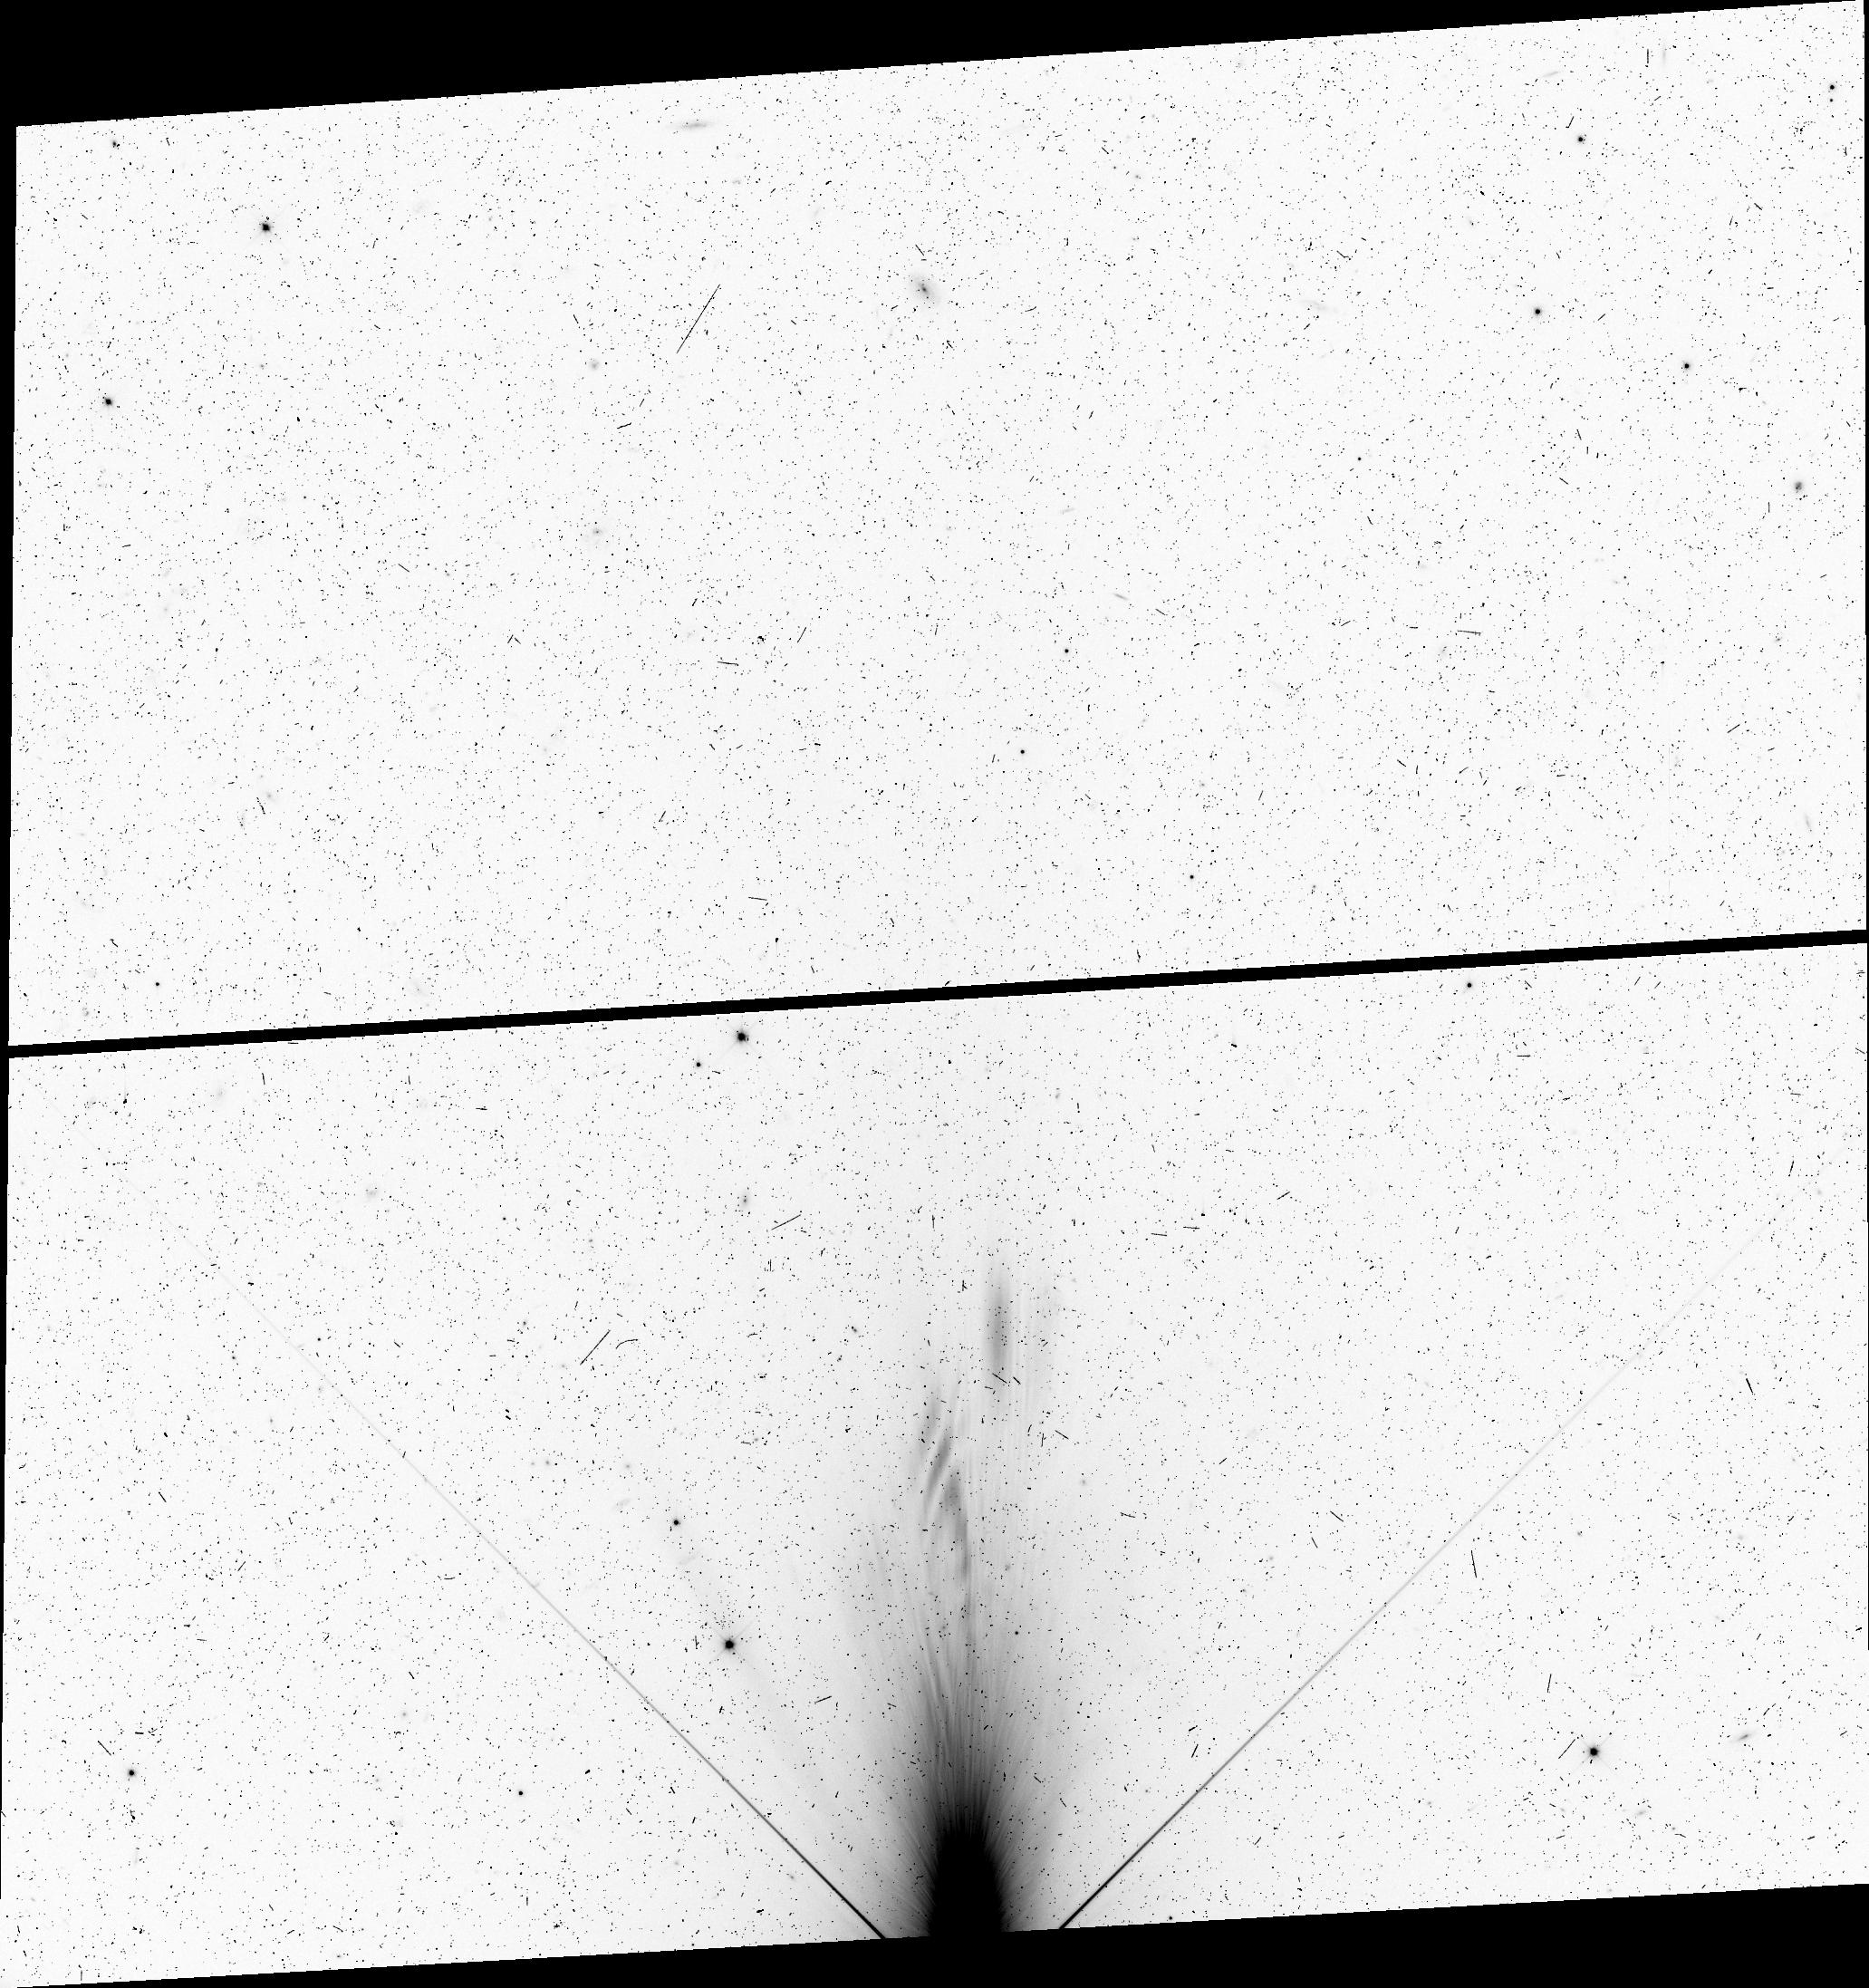
\includegraphics[width=.33\textwidth]{images/not_subtle_dragon.png}}
\mbox{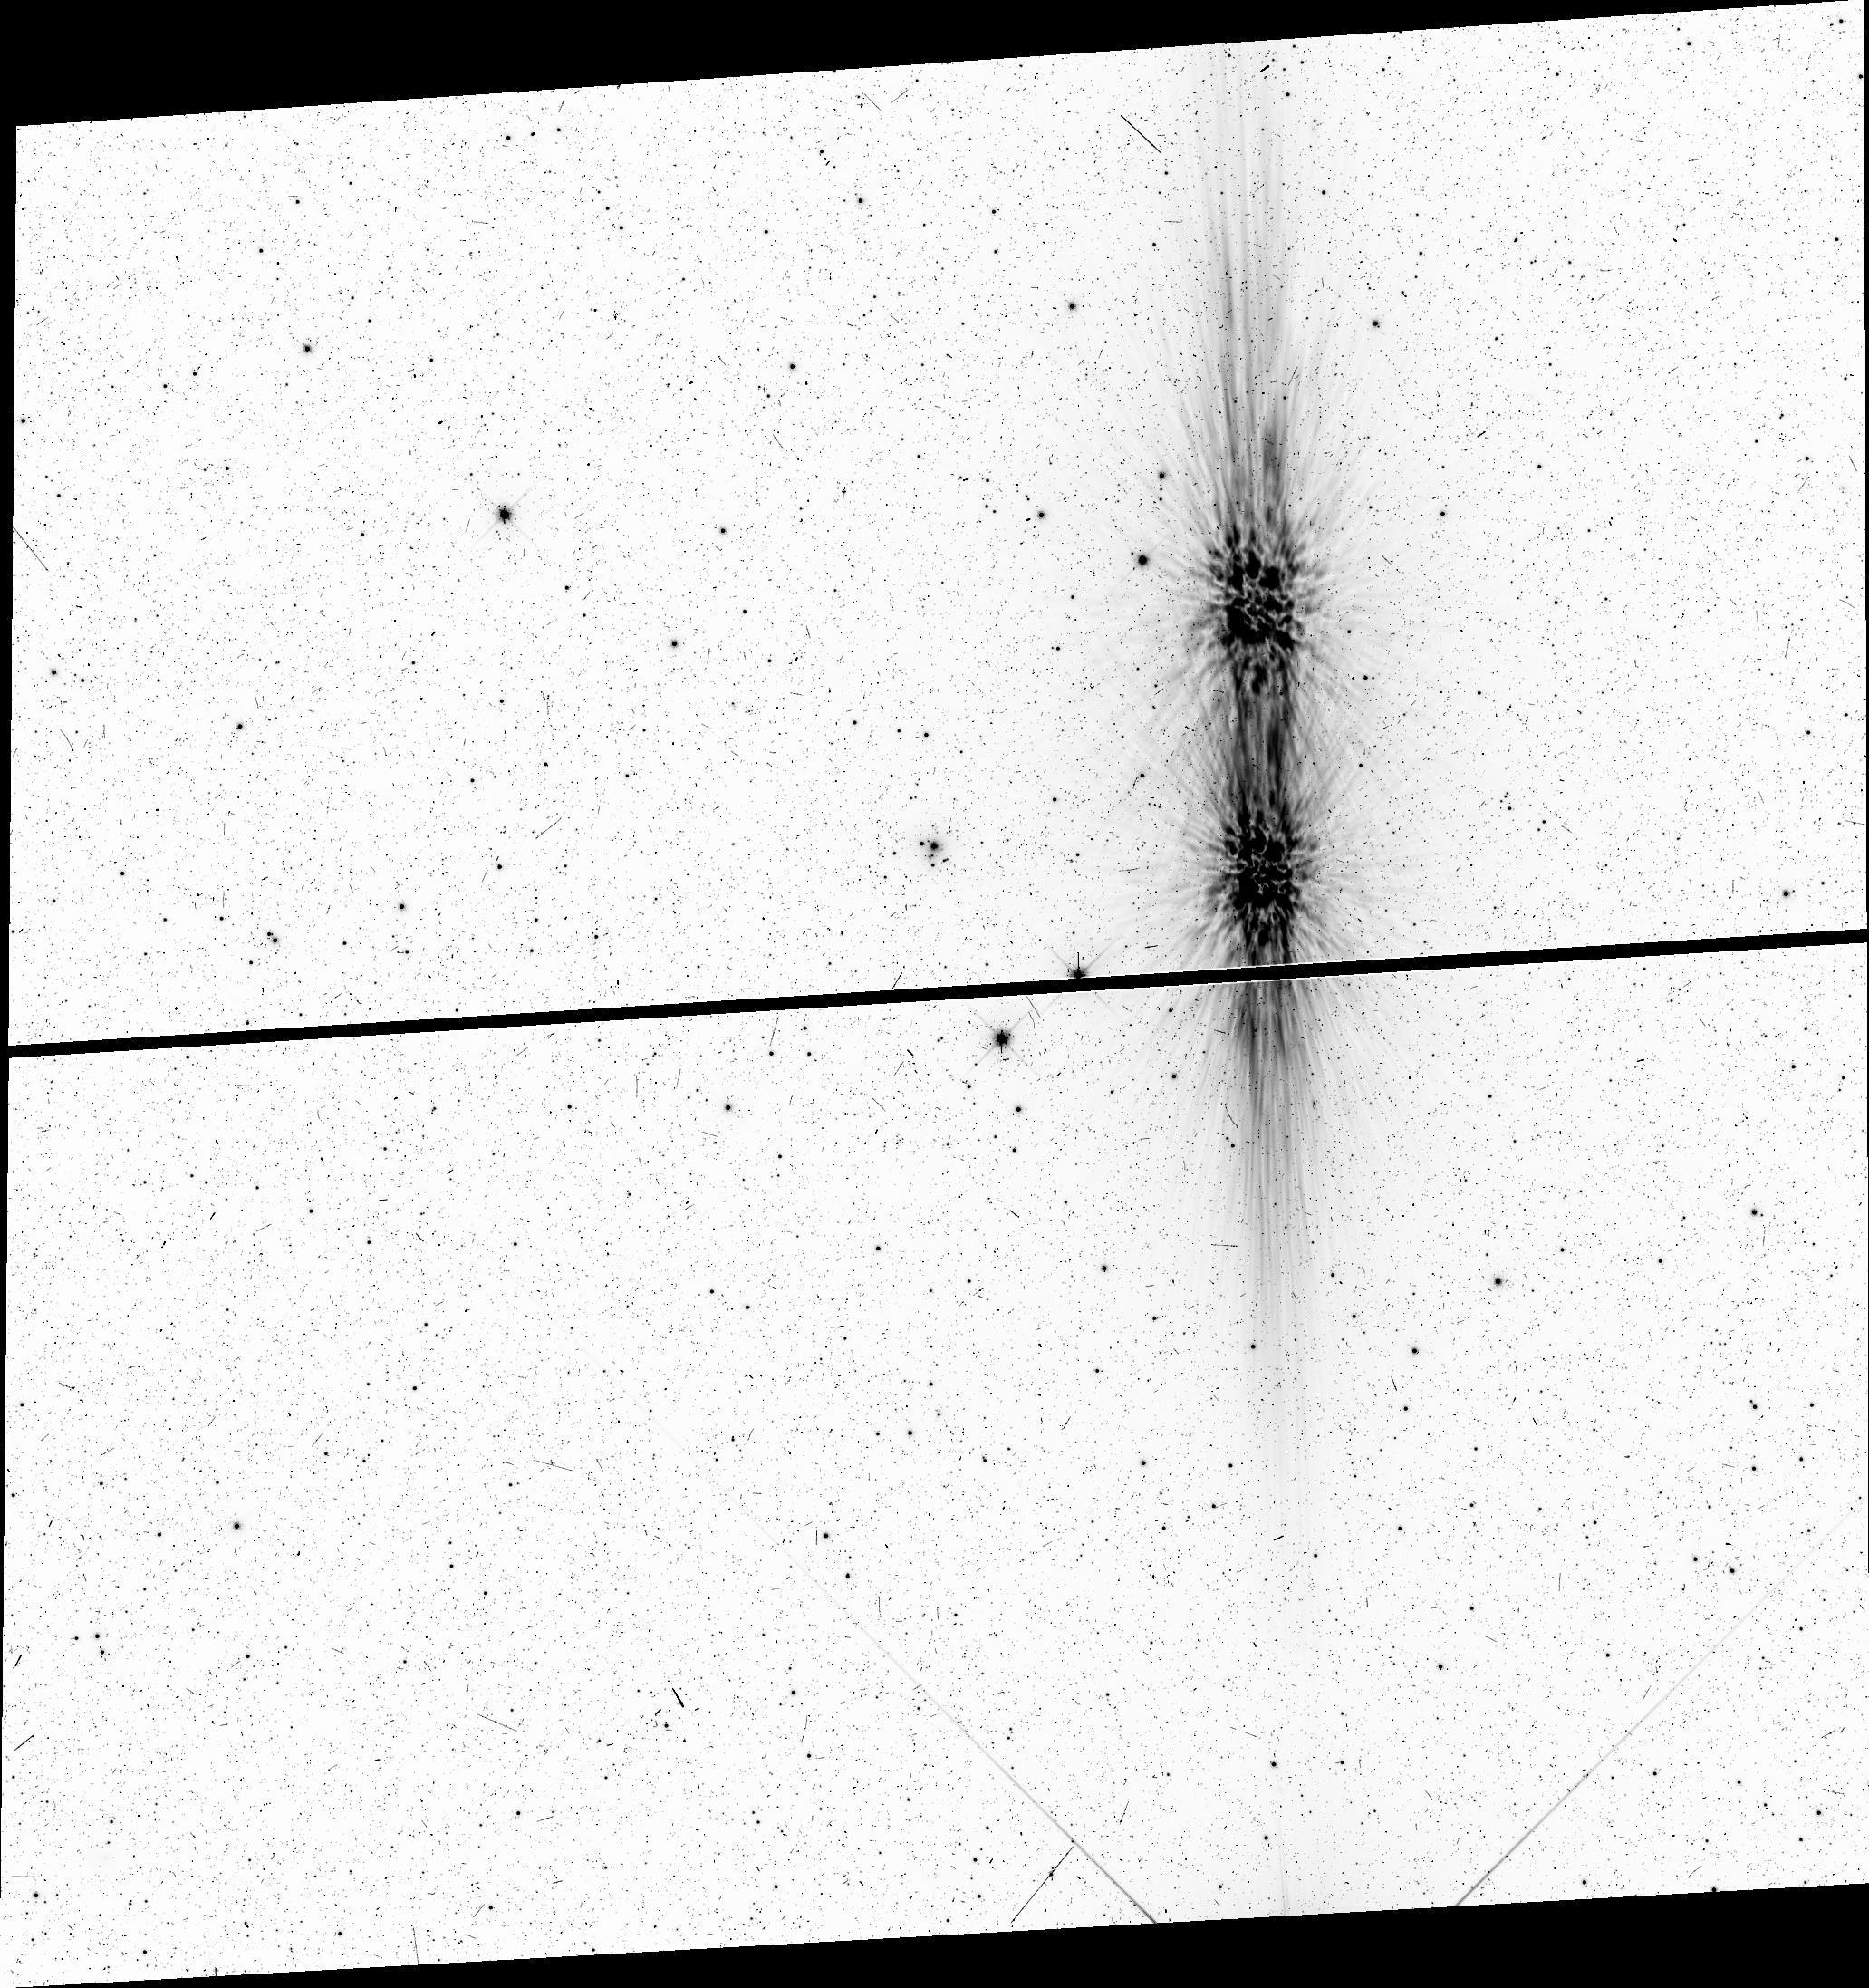
\includegraphics[width=.33\textwidth]{images/scattered.png}}
\mbox{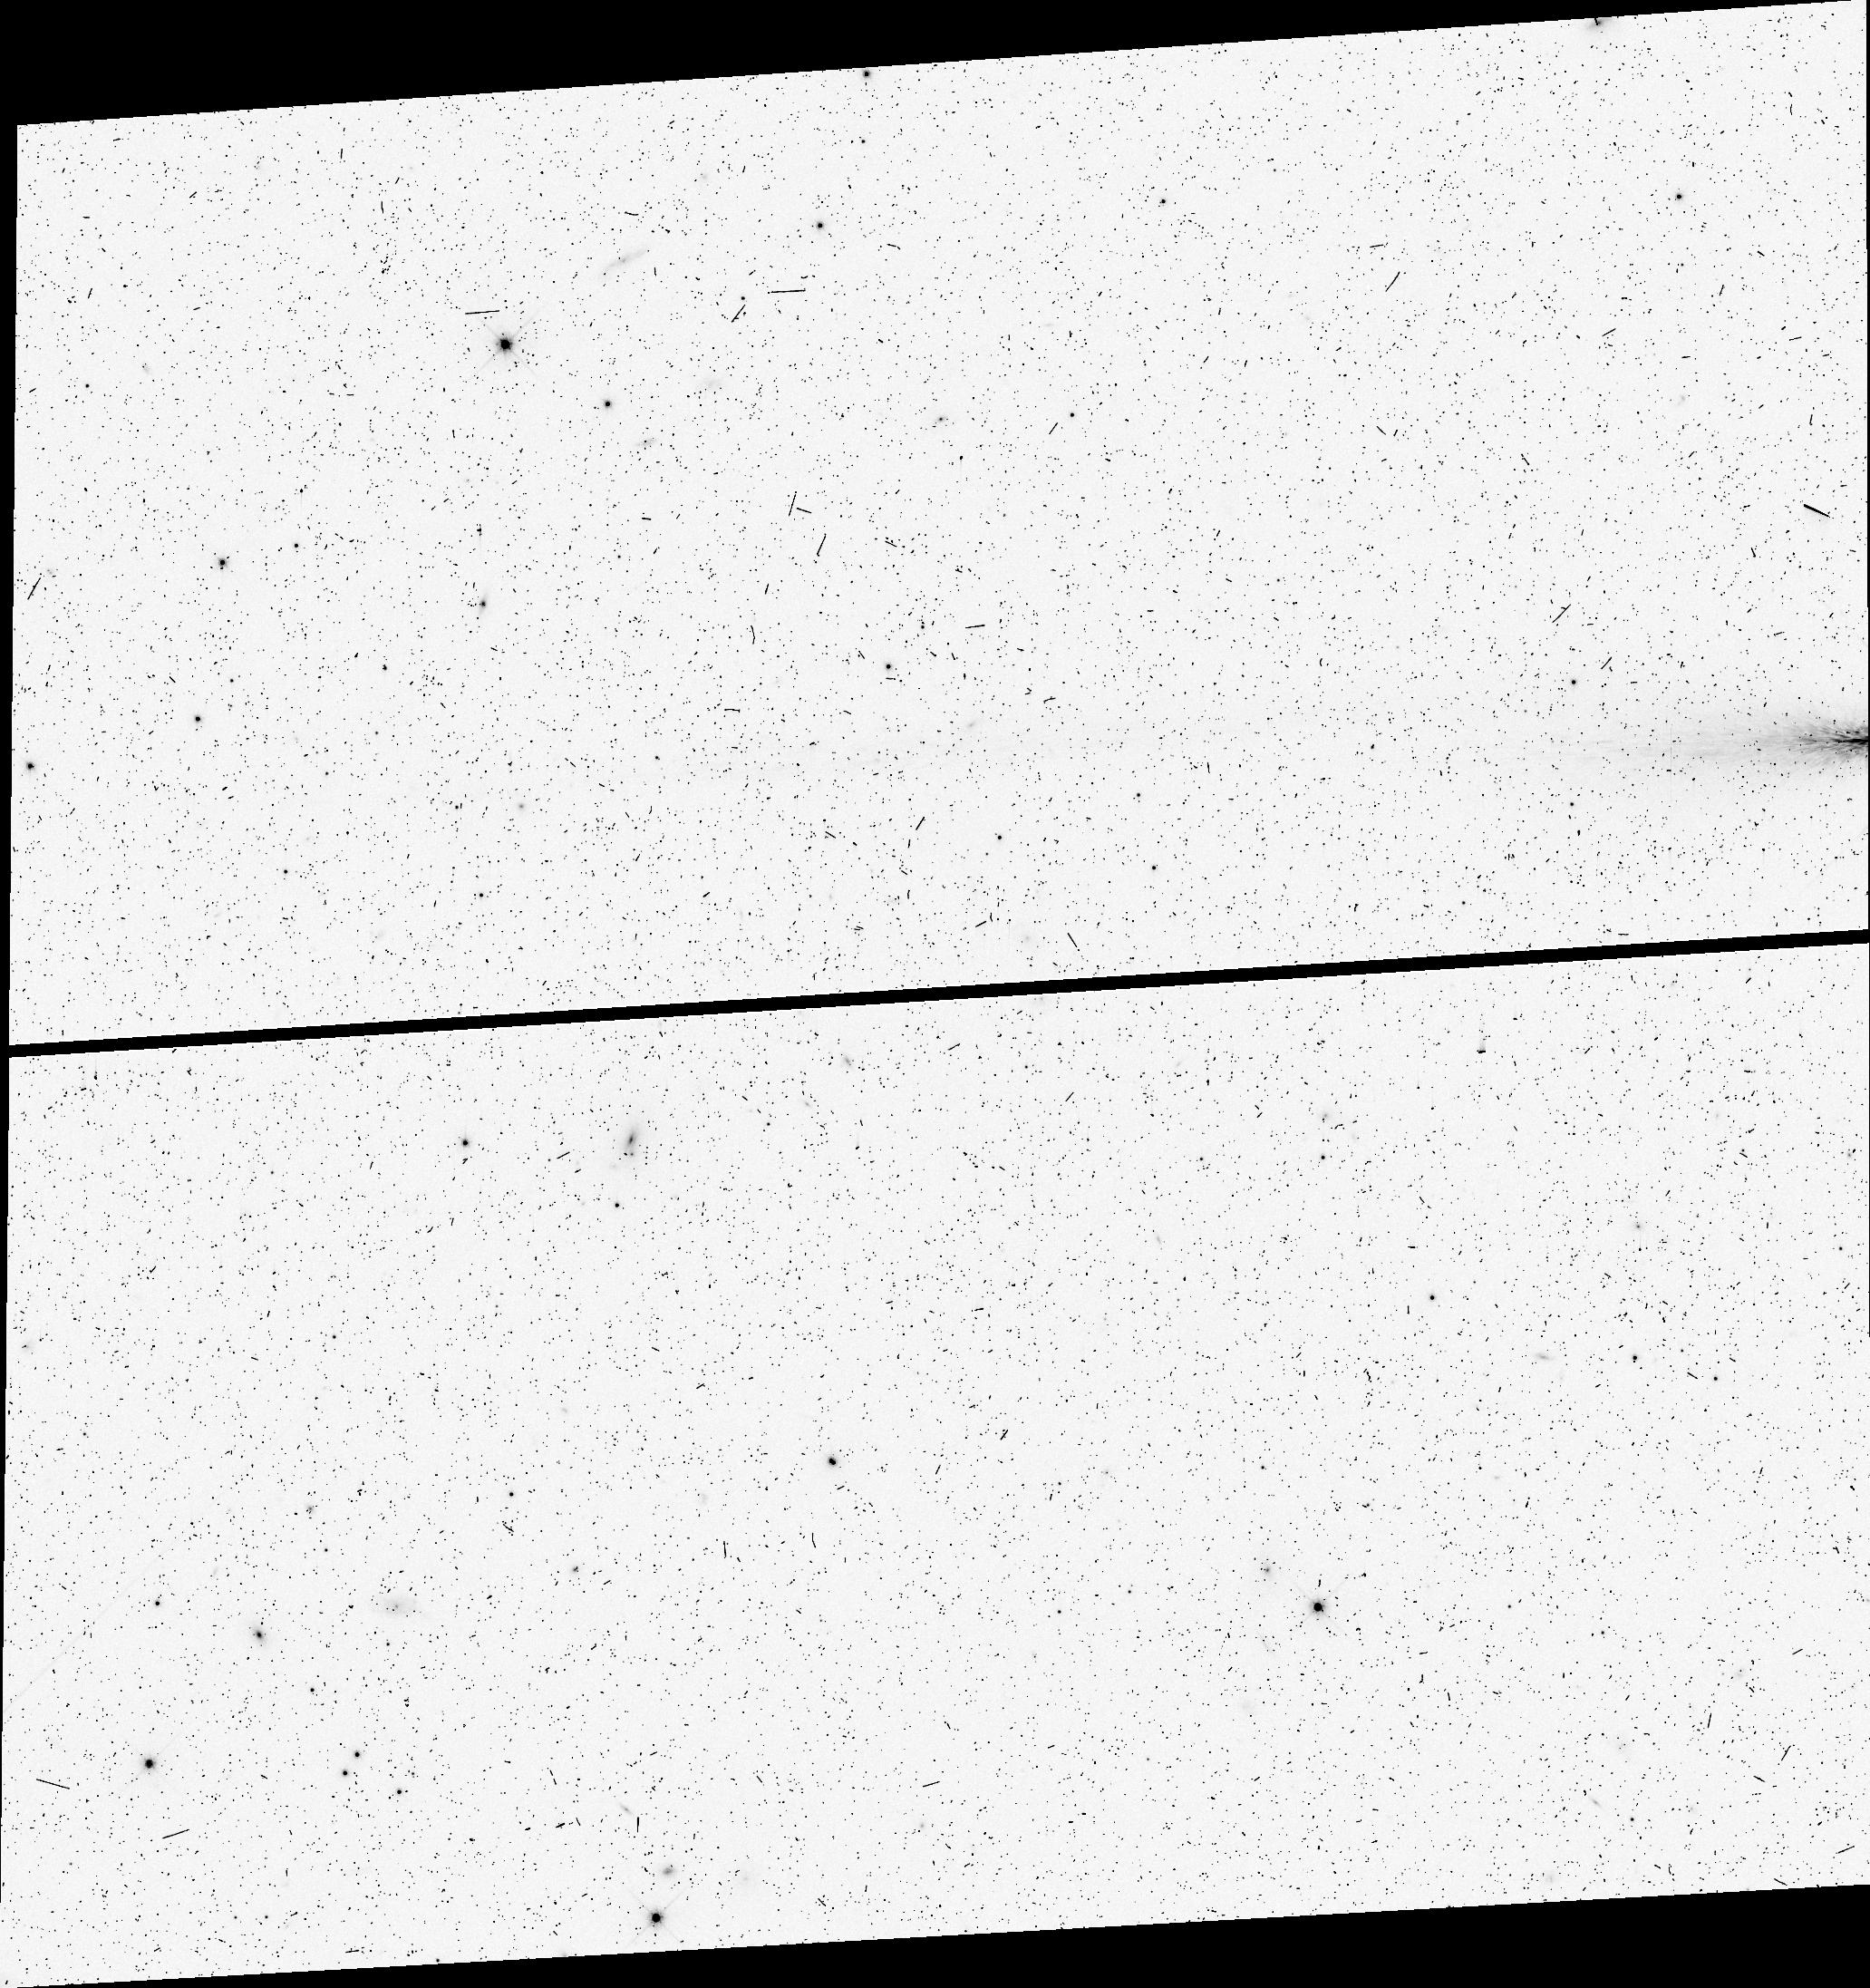
\includegraphics[width=.33\textwidth]{images/subtle_dragon.png}}
}
\caption{\textit{Left: From the bottom of the image a prominent example of Dragon's Breath spills into the image. 
    Middle: In this image a dramatic example of Scattered Light projects an effect into the middle of the detector image.
    Right: A more subtle example of Dragon's Breath from the top right, this resembles the bulk of Dragon's Breath effects.}}
\label{fig:ANOMALIES}
\end{figure}
%fig%%%%-------------------------------------------------------%%%%%%


%tab%%%%-------------------------------------------------------%%%%%%
\begin{table}[h!]
\makebox[\textwidth][c]{
\begin{tabular}{|l|l|l|l|}
\hline
    Effect & Pixels within Region & Mean Pixel Value & Median Pixel Value \\  
\hline
    \rowcolor{gray} Large Anomaly & $1.0\times10^6$ & 130.5 & 59.6  \\ 
    Small Anomaly & $1.1\times10^6$ & 44.9 & 29.2 \\ 
    \rowcolor{gray} No Anomaly & $1.0\times10^6$ & 40.1 & 27.9 \\ 
\hline
\end{tabular}
} 
\caption{\textsl{By comparing the counts in three regions, one entirely made up by an anomaly, 
    one with a small anomaly, and one with just image background, we can quantitatively compare
    the impact of Dragon's Breath on an image.}}
\label{tab:snr_stats}
\end{table}
%tab%%%%-------------------------------------------------------%%%%%%


%%%%%%%%%%%%%%%%%%%%%%%%%%%%%%%%%%%%%%%%%%%%%%%%%%%%%%%%%%%%%%%%%%%%%%%%%%%%%%%%%%%%%%%%%%%
%                                       Data
%%%%%%%%%%%%%%%%%%%%%%%%%%%%%%%%%%%%%%%%%%%%%%%%%%%%%%%%%%%%%%%%%%%%%%%%%%%%%%%%%%%%%%%%%%%

\ssectionstar{Data}
\normalsize{

We began with two data sets on GD-71 and GD-153. Both utilized both IR grisms (G102 and G141) and had matching direct
observations in at least F105 and F140 repsectively, and some with additional matching direct filters F... and F...



{\bf Grism Extraction with \texttt{grizli}}

It is non-trivial to extract these punk grisms. 
...
}
%%%%%%%%%%%%%%%%%%%%%%%%%%%%%%%%%%%%%%%%%%%%%%%%%%%%%%%%%%%%%%%%%%%%%%%%%%%%%%%%%%%%%%%%%%%
%                                   Analysis
%%%%%%%%%%%%%%%%%%%%%%%%%%%%%%%%%%%%%%%%%%%%%%%%%%%%%%%%%%%%%%%%%%%%%%%%%%%%%%%%%%%%%%%%%%%

\ssectionstar{Analysis}
\normalsize{

There are some flux profiles and sensitivity curves...

}

%%%%%%%%%%%%%%%%%%%%%%%%%%%%%%%%%%%%%%%%%%%%%%%%%%%%%%%%%%%%%%%%%%%%%%%%%%%%%%%%%%%%%%%%%%%
%                               Results
%%%%%%%%%%%%%%%%%%%%%%%%%%%%%%%%%%%%%%%%%%%%%%%%%%%%%%%%%%%%%%%%%%%%%%%%%%%%%%%%%%%%%%%%%%%

\ssectionstar{Updates to Flux Extraction and Spectral Trace??}
\normalsize{

I'm honestly not sure at this point if our results will be -- THESE ARE OUR discrepancies
or -- THESE ARE HOW WE FIXED THEM...
}

%%%%%%%%%%%%%%%%%%%%%%%%%%%%%%%%%%%%%%%%%%%%%%%%%%%%%%%%%%%%%%%%%%%%%%%%%%%%%%%%%%%%%%%%%%%
%                                           Acknowledgments 
%%%%%%%%%%%%%%%%%%%%%%%%%%%%%%%%%%%%%%%%%%%%%%%%%%%%%%%%%%%%%%%%%%%%%%%%%%%%%%%%%%%%%%%%%%%
\ssectionstar{Acknowledgements}
\normalsize{
\setlength{\parindent}{0pt}

Whoever edits this?

}
%%%%%%%%%%%%%%%%%%%%%%%%%%%%%%%%%%%%%%%%%%%%%%%%%%%%%%%%%%%%%%%%%%%%%%%%%%%%%%%%%%%%%%%%%%%
%                                            Reference List
%%%%%%%%%%%%%%%%%%%%%%%%%%%%%%%%%%%%%%%%%%%%%%%%%%%%%%%%%%%%%%%%%%%%%%%%%%%%%%%%%%%%%%%%%%%
\newpage
\ssectionstar{REFERENCES}
\normalsize{
\setlength{\parindent}{0pt}

Baggett, S. et al. 2006, Proc. of SPIE, 6265, 626532-2, ``Filters for HST Wide Field Camera 3''

ISR 2016-06: ACS Cycle 24: Here There Be Dragons: Characterization of ACS/WFC Scattered Light Anomalies, B. Porterfield et al. 01 Nov 2016

Lasker, B. et al. 2008, AJ, 136, 735, ``The Second-Generation Guide Star Catalog: Description and Properties''

Skrutskie, M. F. et al. 2006, AJ, 131, 1163, ``The Two Micron All Sky Survey (2MASS)''

The Hubble Space Telescope Wide Field Camera 3 Quicklook Project, Bourque,
Matthew, Bajaj, Varun, Bowers, Ariel, Dulude, Micheal, Durbin, Meredith, Gosmeyer,
Catherine, Gunning, Heather, Khandrika, Harish, Martlin, Catherine, Sunnquist, Ben,
Viana, Alex, ADASS 2016 (proceedings in press)

TIR 2017-01: Aladin Overlay of a Zone of Avoidance for Dragon's Breath, P. R. McCullough 2017 (in prep)

}

%%%%%%%%%%%%%%%%%%%%%%%%%%%%%%%%%%%%%%%%%%%%%%%%%%%%%%%%%%%%%%%%%%%%%%%%%%%%%%%%%%%%%%%%%%%
%                                            Appendix A
%%%%%%%%%%%%%%%%%%%%%%%%%%%%%%%%%%%%%%%%%%%%%%%%%%%%%%%%%%%%%%%%%%%%%%%%%%%%%%%%%%%%%%%%%%%
\newpage
\ssectionstar{Appendix A}
\normalsize{
}

%%%%%%%%%%%%%%%%%%%%%%%%%%%%%%%%%%%%%%%%%%%%%%%%%%%%%%%%%%%%%%%%%%%%%%%%%%%%%%%%%%%%%%%%%%%
%                                        End of Document
%%%%%%%%%%%%%%%%%%%%%%%%%%%%%%%%%%%%%%%%%%%%%%%%%%%%%%%%%%%%%%%%%%%%%%%%%%%%%%%%%%%%%%%%%%%
\clearpage
\end{document}
